\documentclass[11pt]{article}

\usepackage[a4paper,margin=1in]{geometry}
\usepackage[T1]{fontenc}
\usepackage{newtxtext,newtxmath}
\usepackage{microtype}
\usepackage{amsmath}
\usepackage{graphicx}
\usepackage{booktabs}
\usepackage{threeparttable}
\usepackage{caption}
\usepackage{setspace}
\usepackage{enumitem}
\usepackage[dvipsnames]{xcolor}
\usepackage{tikz}
\usetikzlibrary{arrows.meta,positioning}
\usepackage{xurl}
\usepackage[round,authoryear]{natbib}
\usepackage[colorlinks=true,linkcolor=MidnightBlue,citecolor=MidnightBlue,urlcolor=MidnightBlue]{hyperref}
\hypersetup{pdftitle={Information versus Enforcement against Greenwashing: Pre-Registered Experiments in a Multi-Agent Artificial Market}, pdfauthor={Ellis Lin}, pdfkeywords={greenwashing, ESG disclosure, agent-based model, inspection game, impact investing, audit targeting, pre-registration}}

% Marked placeholders: visible in the PDF so nothing pending is circulated by accident.
\newcommand{\pending}[1]{\textcolor{BrickRed}{[Pending: #1]}}
\newcommand{\fillin}[1]{\textcolor{BrickRed}{[#1]}}
\newcommand{\Vh}{V\textsubscript{hidden}}
\newcommand{\Jh}{J\textsubscript{hidden}}

\setstretch{1.12}
\captionsetup{font=small,labelfont=bf}
\setlist{itemsep=2pt,topsep=4pt}
\newtheorem{proposition}{Proposition}
\newenvironment{proofsketch}{\par\noindent\textit{Proof.}\ }{\hfill$\square$\par}

\title{Information versus Enforcement against Greenwashing:\\[2pt]
Pre-Registered Experiments in a Multi-Agent Artificial Market}
\author{Ellis Lin\thanks{Fudan University. E-mail: \href{mailto:kanzaler123@gmail.com}{kanzaler123@gmail.com}. Preliminary; comments welcome. Code, configuration files, the pre-registrations and all evidence are at \url{https://github.com/kanzaler123/financial-ABM}. An in-browser version of the firm decision layer is at \url{https://kanzaler123.github.io/financial-ABM/}.}}
\date{This version: 20 October 2026}

\begin{document}
\maketitle

\begin{abstract}
\noindent Regulators can fight greenwashing by making inflated disclosures easier to see through or by fining them when audits detect them. We compare the two in an agent-based artificial market where 1,000 investors trade the shares of 200 firms. Impact investors value reported ESG scores, and investors switch types by imitation. Every period each firm chooses between costly real improvement, cheap inflation of its report that audits may detect, and doing nothing; a regulator sets transparency, audits and fines. The market is initialised on CSI~300 constituents, investor taste is calibrated to an ESG cost-of-capital slope of about 28 basis points per standard deviation, and the baseline fine is China's statutory maximum of CNY~10 million per case. In a pre-registered experiment of 59 scenarios with 30 paired seeds each: (i) policies work only through investor preference, without which firms neither improve nor inflate; (ii) raising transparency from 0.1 to 0.6 raises the true ESG level more than quadrupling the fine, and both beat the baseline, both without natural decay of the true level and at 0.2 standard deviations (SD) per year; the effect of transparency against the baseline is $+0.04$ and $+0.33$~SD at these two uncalibrated rates; (iii) fixed fines lose deterrence quickly because inflation added to an undetected case is not fined again, and they leave large firms, for which CNY~10 million is negligible, inflating in 66\% of their decisions. Exploratory supplements designed after these results keep the ordering at three intermediate decay rates, when true levels revert to the mean, when every false report is fined, and when washing costs differ across firms. But the size of the information advantage depends on two assumptions. Under mean reversion at rates bounded by a rating panel, transparency beats the quadrupled fine by only $+0.003$ to $+0.006$~SD, because improvements fade while inflation persists. With a fine for every false report, the gap shrinks from $+0.205$ to $+0.058$~SD, and the plateau in fine deterrence disappears. With firm-specific washing costs, greenwashing declines gradually with transparency instead of stopping at a threshold. Market feedback strengthens the fixed-fine effect by about 11\% and has no identifiable net effect on transparency. A tabular Q-learner trained on realised accounts did not reach a usable policy. A second pre-registered experiment holds the expected number of audits fixed. Auditing in proportion to market value or after jumps in reported scores does worse than random audits when firms know the rule ($-0.19$ and $-0.14$~SD): value targeting moves greenwashing from large to small firms, and firms keep new inflation below the jump threshold. With the rule hidden, neither differs from random audits. All results are conditional on the model.

\medskip
\noindent\textbf{AI disclosure:} The simulation code, the analysis scripts and drafts of this paper were written with the assistance of Claude (Anthropic), an AI model, used through Claude Code. The author directed the research, reviewed all AI-assisted output and is responsible for the content.

\medskip
\noindent\textbf{Keywords:} greenwashing; ESG disclosure; agent-based model; inspection game; impact investing; audit targeting; pre-registration.\\
\noindent\textbf{JEL:} C63, G18, G23, K22, K42, M14, Q56.
\end{abstract}

\newpage

%======================================================================
\section{Introduction}
%======================================================================

A firm that reports better environmental, social and governance (ESG) performance than it delivers can be met with two kinds of regulatory response. An \emph{information} policy makes inflated claims easier to see through: standardised metrics, third-party assurance or published audit results reduce the share of an inflated report that investors take at face value. An \emph{enforcement} policy leaves visibility unchanged and raises the price of being caught. Both are open questions in China. Exchange guidelines issued in 2024 require several hundred large listed companies to publish sustainability reports from the 2025 reporting year, but they provide only self-regulatory measures and disciplinary sanctions for violations \citep[e.g.][]{sse2024guideline}. The Securities Law caps the fine for false disclosure at CNY~10 million per case \citep{securitieslaw2019}, about 0.01\% of the median market value of a CSI~300 constituent, and it is not settled whether the provision reaches ESG reports at all.

Which instrument moves real ESG performance more is hard to learn from data. Neither has been applied to ESG reports at scale, true performance is not observed, and the effect of either depends on how investors price reported scores, which depends in turn on how many investors care about them. We therefore study the question in a computational laboratory: an artificial stock market in which investors, firms and a regulator interact, initialised and calibrated to Chinese magnitudes, and in which a policy can be switched on in otherwise identical worlds.

The model has three layers (Section~\ref{sec:model}). Impact investors add a taste for reported ESG to a mean--variance utility, so a better reported score raises a firm's price and lowers its financing cost; the population of investors evolves by pairwise imitation \citep{schlag1998imitate}. Every sixty trading days each of 200 firms chooses between costly real improvement, which takes effect with a delay, cheap inflation of its report, which an audit may detect, and doing nothing. Firms decide by a net-present-value (NPV) rule that prices the financing gain the market would grant. A regulator sets transparency, the audit probability and fines. The firm layer has a closed-form benchmark (Section~\ref{sec:benchmark}): an inspection game \citep{avenhaus2002inspection} whose two propositions give the condition for inflating under a lump-sum fine and a transparency threshold above which no firm inflates. Unlike the closest agent-based work on green disclosure \citep{zhao2025agent,zhao2026green}, in which greenwashing arises passively from pooled disclosure categories, our firms choose how much to misreport, face audits and fines booked per case, and differ in size, and the market they finance themselves in responds to policy.

The experiment was pre-registered (Section~\ref{sec:design}). Design, seeds, metrics, four primary questions and the analytical predictions were committed to the public repository before the confirmatory run of 59 scenarios with 30 paired seeds each, 1,770 simulated markets of 3,500 trading days. Analyses designed after seeing the results are labelled exploratory, and each was itself written down before it was run. A second experiment, on targeted audits, was pre-registered in the same way and run on new seeds (Section~\ref{sec:targeted}).

Six findings stand out (Sections~\ref{sec:results}--\ref{sec:targeted}).
\begin{enumerate}[leftmargin=*]
\item \emph{Policy works only through investor preference.} Impact investors' taste raises the true ESG level by 0.79 standard deviations (SD) over the full fourteen years. Without it, firms neither improve nor inflate, and none of the policies has any effect.
\item \emph{At the tested doses, information beats enforcement.} Raising transparency from 0.1 to 0.6 raises the true level more than quadrupling the fixed fine, and both beat the baseline. The ordering holds at both pre-registered rates of natural decay of the true level, none and 0.2~SD per year, and at three intermediate rates added in an exploratory supplement; the magnitudes do not. The effect of transparency against the baseline is $+0.04$~SD without decay and $+0.33$~SD at 0.2~SD per year, and decay is the model's most important uncalibrated parameter.
\item \emph{Fixed fines lose deterrence quickly and miss large firms.} Moving from no fine to the statutory CNY~10 million cuts the share of decisions that inflate from 91\% to 22\%, but eight times that fine still leaves 12.5\%, because inflation added to an undetected case incurs no new fine. The fine is negligible against the value of large firms, which inflate in 66\% of their decisions against 6\% for small firms. A fine proportional to market value reverses this size pattern but, at an equal-amount reference, leaves far more inflation overall.
\item \emph{The ordering is robust; the size of the information advantage is not} (exploratory). The ordering survives every setting tested, but the advantage of transparency over the quadrupled fine falls to $+0.003$--$+0.006$~SD when true levels revert to the mean at rates bounded by a rating panel: improvements fade while inflation persists, which lifts the transparency threshold above 0.6. It falls to $+0.058$~SD when every false report is fined, which also removes the plateau in fine deterrence (8 times the fine then leaves 0.8\% of decisions inflating). With firm-specific washing costs the comparison is unchanged, but inflation declines gradually with transparency instead of stopping at a threshold.
\item \emph{Market feedback is modest and runs in both directions} (exploratory). Replaying the firms' decisions on the baseline run's financing gains and market values isolates the feedback from policy to prices, financing gains and the investor population. In the main setting it strengthens the fixed-fine effect by about 11\% and narrows the gap between the instruments by about 10\%; its net effect on the transparency policy cannot be distinguished from zero, because investor evolution weakens that policy while price responses strengthen it. When investor taste is doubled, feedback accounts for 31\% of the fixed-fine effect.
\item \emph{Targeted audits backfire when firms know the rule} (second experiment). At an unchanged expected number of audits, auditing in proportion to market value lowers the true level by 0.19~SD relative to random audits, and auditing firms whose reports jump lowers it by 0.14~SD, although both rules find inflation more often. Value targeting moves greenwashing from large firms to the more numerous small firms, whose audit rate falls, and firms keep new inflation below the jump threshold. With the rule hidden, neither rule differs from random audits, and doubling random audits raises the true level by 0.12~SD. On the new seeds, information beats the quadrupled fine by $+0.191$~SD, close to the first experiment's $+0.205$.
\end{enumerate}

We are explicit about what the simulation does not show. Most qualitative results follow from the firms' decision rule, which the propositions describe; the artificial market supplies the financing gains that set the magnitudes and measures the feedback. The comparison is at fixed doses, not at equal social cost, because the costs of transparency are not modelled. And a tabular Q-learner \citep{watkins1992qlearning} trained on firms' realised accounts did not reach a usable policy. In our calibration the value of the best action over doing nothing is about 0.07 basis points of market value, while the discounted reward that follows a decision varies with an SD of about 190 basis points within a state. We report this negative result because it limits what the model can say about boundedly rational firms; it does not show that real firms cannot learn the financial value of ESG.

Section~\ref{sec:literature} relates the paper to existing work. Sections~\ref{sec:model}--\ref{sec:design} present the model, the analytical benchmark and the design; Section~\ref{sec:results} reports results; Section~\ref{sec:validity} collects the robustness checks and threats to validity; Section~\ref{sec:targeted} reports the experiment on targeted audits; Section~\ref{sec:conclusion} concludes.

%======================================================================
\section{Related literature}\label{sec:literature}
%======================================================================

\paragraph{Greenwashing and ESG disclosure.} \citet{lyon2011greenwash} model greenwash as selective disclosure by a firm that an activist may audit, and \citet{delmas2011drivers} and \citet{lyon2015means} review its drivers and forms. Empirically, firms both exaggerate and understate their sustainability performance \citep{kim2015greenwash}, and selective disclosure is less common where firms face more scrutiny \citep{marquis2016scrutiny}. On disclosure mandates, \citet{christensen2021mandatory} review the economics of mandatory sustainability reporting; \citet{chen2018effect} find that China's 2008 mandate lowered the profitability of affected firms and reduced pollution in the cities most exposed to them; \citet{fiechter2022real} find that the EU directive raised affected firms' CSR activity. ESG ratings of the same firm diverge widely across providers \citep{berg2022aggregate}, one reason we treat the reported score as a proxy rather than the true attribute. Our information instrument is a stylised version of these mechanisms; unlike reduced-form studies, we can switch it on in otherwise identical markets and compare it with fines.

\paragraph{Enforcement.} The deterrence logic of fines goes back to \citet{becker1968crime}; inspection games formalise the interaction of an inspector who audits with some probability and an inspectee who may violate \citep{avenhaus2002inspection}. We use the inspectee's side as an analytical benchmark for the firm layer. The audit probability in our model is an assumption; as background, \citet{dyck2024pervasive} estimate that only about a third of corporate fraud is detected.

\paragraph{Sustainable investing and the cost of capital.} When some investors exclude polluting firms, those firms' cost of capital rises and they may reform \citep{heinkel2001effect}; in equilibrium, investors' taste for green holdings lowers the expected returns of green assets \citep{pastor2021sustainable,pedersen2021responsible}. Empirical estimates of the financing effect range from 7--18 basis points on US bank loans \citep{goss2011impact} to about 0.19 percentage points of the cost of equity per rating notch for Chinese listed firms \citep{zhao2024esg}, which we use as the calibration target. In our model the premium is both the reward for real improvement and the reward for greenwashing, and the share of investors who pay it evolves.

\paragraph{Agent-based models of green disclosure.} The closest work is by \citet{zhao2025agent} and \citet{zhao2026green}. They simulate firms at three green levels that compete for a fixed pool of ESG fund capital allocated by investors' valuation of each level, and they use empirical game-theoretic analysis to find equilibrium upgrade strategies under strict and lax disclosure and under a two-stage policy that switches from lax to strict. The journal version extends it to a dual-market model of the EU and China. In their model a firm decides only whether to upgrade. Greenwashing is passive: lax disclosure pools low- and high-green firms at their average valuation, and no firm chooses to misreport. There are no audits or fines, and firms differ by green level rather than size. Our paper differs in four respects. Firms actively choose how much to inflate a report, at a cost and under a risk of detection. Enforcement has an explicit audit-and-penalty structure, in which fines are booked per case, fixed and proportional fines are compared, and the statutory cap is calibrated. Firm size matters because a lump-sum fine shrinks relative to value as firms grow, which produces the size divide of Section~\ref{sec:size}. And financing gains come from a market whose prices and investor population respond to policy, so we can measure how much that feedback contributes (Section~\ref{sec:feedback}). Their method answers a question our simulation does not: it builds an empirical payoff table from simulations and applies $\alpha$-Rank, which ranks strategy profiles by their weight in the stationary distribution of an evolutionary dynamic, so it says which profiles a population of firms would persist in.

\paragraph{Agent-based finance and research practice.} Artificial stock markets with heterogeneous, adaptive agents go back to \citet{arthur1997asset}; \citet{lebaron2006agent} surveys the field and \citet{farmer2009economy} argue for its use in policy analysis. We parameterise demand elasticities in the range of the demand-system literature \citep{koijen2019demand} and describe the model following the logic of the ODD protocol \citep{grimm2020odd}. Agent-based studies leave many choices to the researcher; following the case for pre-analysis plans in economics \citep{olken2015promises}, we fixed design, seeds and inference before the confirmatory run and keep failed runs in the record.

%======================================================================
\section{The model}\label{sec:model}
%======================================================================

\subsection{Overview and timing}

A simulation runs for 3,500 trading days (252 per year, about 14 years). Day~0 initialises the market; days 1--1200 are a pre-policy period under the baseline regime; a policy, if any, switches on at day 1201 and stays in place. Outcomes are measured over the policy window, days 1200--3500. The agents are 1,000 investors of two types, 200 firms in three size tiers (the largest 10\%, the next 30\% and the remaining 60\% by initial value), market makers with an aggregate noise-trader account, and a regulator. Figure~\ref{fig:schematic} shows how they interact. Table~\ref{tab:parameters} lists the main parameters with their sources.

\begin{figure}[t]
\centering
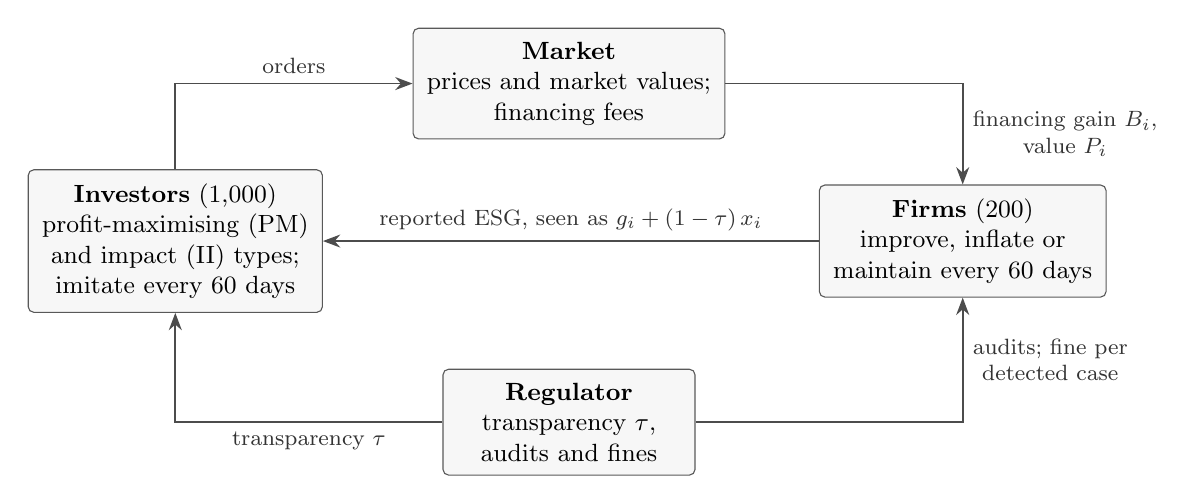
\begin{tikzpicture}[
  box/.style={draw=black!65, fill=black!3, rounded corners=2pt, align=center, font=\small, inner sep=5pt, minimum width=3.2cm},
  arr/.style={-{Stealth[length=2.2mm]}, draw=black!70, line width=0.6pt},
  lab/.style={font=\footnotesize, align=center, text=black!80}]
\node[box] (inv) at (0,0) {\textbf{Investors} (1,000)\\profit-maximising (PM)\\and impact (II) types;\\imitate every 60 days};
\node[box] (mkt) at (5.0,2.0) {\textbf{Market}\\prices and market values;\\financing fees};
\node[box] (firm) at (10.0,0) {\textbf{Firms} (200)\\improve, inflate or\\maintain every 60 days};
\node[box] (reg) at (5.0,-2.3) {\textbf{Regulator}\\transparency $\tau$,\\audits and fines};
\draw[arr] (inv.north) |- node[lab, pos=0.75, above] {orders} (mkt.west);
\draw[arr] (mkt.east) -| node[lab, pos=0.75, right] {financing gain $B_i$,\\ value $P_i$} (firm.north);
\draw[arr] (firm.west) -- node[lab, above] {reported ESG, seen as $g_i + (1-\tau)\,x_i$} (inv.east);
\draw[arr] (reg.east) -| node[lab, pos=0.75, right] {audits; fine per\\ detected case} (firm.south);
\draw[arr] (reg.west) -| node[lab, pos=0.25, below] {transparency $\tau$} (inv.south);
\end{tikzpicture}
\caption{Structure of the model. A firm's true level is $g_i$ and its undetected inflation $x_i$; investors see the inflation only in part, $1-\tau$. Firms affect each other and are affected by investors only through the financing gain $B_i$ and their market value $P_i$.}
\label{fig:schematic}
\end{figure}

\subsection{Firms and the disclosure state}

Each firm $i$ has a latent true level $g_i$, measured in units of its initial cross-sectional standard deviation (SD), and undetected inflation $x_i \ge 0$; its report is $g_i + x_i$. Investors observe the signal
\begin{equation}
s_i = \min\{\, g_i + (1-\tau)\,x_i,\; C \,\},
\label{eq:signal}
\end{equation}
where $\tau \in [0,1]$ is transparency, the share of inflation that investors see through, and $C$ is the latent value of a perfect score of 100 points. Reports cannot exceed a perfect score, so inflation is capped at $\max\{C - g_i, 0\}$. Without effort, the true level decays by $\delta$~SD per year (main setting $\delta = 0.2$).

Every 60 trading days each firm takes one of three actions. \emph{Improve} by $\Delta$ costs $c_i\Delta^2$ and raises $g_i$ after an implementation delay of 120 days. \emph{Inflate} by $\Delta$ costs $w\,c_i\Delta^2$ and enters the published report after 20 days. \emph{Maintain} costs nothing. Changes are capped at 0.25~SD per period. Improvement beyond the report's remaining room replaces inflation, so only its transparent share is newly visible. The marginal cost scale is $c_i = \bar c\, m_{k(i)}\, \varepsilon_i\, e^{\eta g_i}$, with $\bar c = 0.05$, size multipliers $m = (0.6, 1, 1.6)$ for large, mid and small firms, lognormal dispersion $\varepsilon_i$ with log-SD 0.5, and $\eta = 1.5$, so improvement becomes dearer as the level rises. The size multipliers assume that large firms improve more cheaply; an equal-cost control removes them. The washing cost ratio $w = 0.2$ has no empirical basis and is varied in the experiment. Costs, fines and subsidies change a firm's intrinsic value and reach its price through the market makers on the next day.

\subsection{Investors and prices}

Investors differ in wealth (lognormal), risk aversion $\gamma_j$ and decision calendar (median 20 days). On a decision day an investor sets its equity share to the Merton ratio $(E[R_m]-r_f)/(\gamma_j \sigma_m^2)$, clipped to $[0,1]$, and allocates equity across firms by a softmax tilt away from market weights,
\begin{equation}
w_{ji} \propto P_i \exp(\kappa_j U_{ji}), \qquad U_{ji} = E[R_i] - \gamma_j\,\mathrm{cov}(r_i, r_m) + \theta_j\, s_i ,
\label{eq:utility}
\end{equation}
moving half-way from its current to its target holdings. Profit-maximising investors (PM) have $\theta_j = 0$. Impact investors (II) have a lognormal taste $\theta_j$, measured as an annual-return equivalent per SD of the signal, with median $\bar\theta$ and log-SD 0.5. With equal utilities every investor holds the market portfolio, which keeps the rule consistent with a fixed supply of shares.

Each firm's shares are quoted by a market maker who passes through news about intrinsic value and moves the price with order flow. Price impact has a permanent and a transient part, depth thins when volatility rises, and an aggregate noise-trader account adds correlated flow. Seven market parameters were fitted by the method of simulated moments to return moments of US industry portfolios; cash and shares are conserved every day. The market layer was frozen before any policy experiment, and its known defects are reported in Section~\ref{sec:validity}.

\subsection{Investor evolution}

Every 60 days, 10\% of investors review their type. Each reviewer samples one other investor uniformly; if the partner is of the other type, the reviewer switches with probability $k \cdot \max\{0, \bar G_{\text{other}} - \bar G_{\text{own}}\}$, where $\bar G$ is the mean wealth growth of each type over the window and $k = 100$. This is the proportional imitation rule of \citet{schlag1998imitate}. The expected change in the impact-investor share $s$ is $m\,k\,s(1-s)\,E[\bar G_{II} - \bar G_{PM}]$ with review share $m$, a discrete replicator dynamic \citep{taylor1978evolutionary}, so the share does not drift when the two types perform equally. An earlier implementation omitted the partner draw and drifted towards one half even at zero taste. With the corrected rule, the change in the share over 14 years at zero taste has 95\% intervals that include zero at initial shares of 0.2, 0.5 and 0.8 (20 seeds each), and a taste near the calibrated value raises it by 2.3 percentage points [1.4, 3.1] from an initial share of 0.2: the market's own drive towards impact investing is small.

\subsection{Financing gains and the firm's decision rule}

Each firm has a fixed external financing exposure $E_i$, half of its initial market value, whose fee rate $r_f + 0.05\, E_i/(E_i + P_i^{\text{lag}})$ is repriced every 60 days. A firm estimates the local permanent response of its price to its own signal, holding everything else fixed, and converts it into $B_i$, the annual financing saving per SD of signal as a share of current market value. Discounting at 5\% a year, the calendar of delays, repricing dates and audits gives three factors. The signal annuities of real improvement, $A_r$, and of inflation, $A_w$ (which lasts only until an audit), count financing savings over a five-year horizon. The expected discounted value $D$ of paying one unit when new inflation is detected has no horizon: a false report remains a liability until an audit finds it, so $D$ sums the audit probability over all future audit dates. With subsidy $\sigma$ per SD, proportional fine $p$ per SD of detected inflation, fixed fine $F$ and market value $P$, the values of the three actions are
\begin{align}
V_I &= \frac{(B A_r + \sigma)^2}{4c}, \label{eq:vi}\\
V_W &= \frac{\max\{B(1-\tau)A_w - pD,\, 0\}^2}{4wc} - \pi \frac{F}{P} D, \label{eq:vw}\\
V_M &= 0, \nonumber
\end{align}
with optimal sizes $(BA_r+\sigma)/2c$ and $(B(1-\tau)A_w - pD)/2wc$ before caps. The term $\pi$ is the probability that new inflation opens a new case, which is zero for a firm that already carries undetected inflation (see below). The firm takes the action with the highest value and maintains on ties. The rule is myopic: firms re-optimise every period and do not anticipate their own future choices.

\subsection{The regulator}

In each 60-day period every firm is audited with probability 1\%. An audit that finds inflation opens a case: the firm pays the fixed fine $F$ plus $p$ times its inflation, and the inflation is removed. Inflation added while earlier inflation is still undetected joins the same case and adds no fixed fine. We call this \emph{per-case booking}; the alternative, a separate fine for every false report, is not implemented and is discussed in Section~\ref{sec:validity}. In the main setting $p = 0$ and $F$ equals CNY~10 million, the statutory maximum, which is $4.56\times10^{-5}$ of the average firm's initial value. Baseline transparency is $\tau = 0.1$. The second experiment (Section~\ref{sec:targeted}) replaces random audits with targeted rules.

\subsection{Initialisation and calibration}

The market is initialised on the CSI~300 constituents of 9 October 2026, matched 300 of 300 on Huazheng composite ESG scores, half-year book equity and market value (Table~\ref{tab:parameters}). Scores are mapped to the latent standard-normal level by their empirical quantiles, so the scale saturates at a perfect score, and the latent level is linked to log value by a Gaussian copula with $\rho = 0.177$, converted from the sample Spearman correlation of 0.169. The dispersion of log intrinsic value, 0.915, is the cross-sectional SD of log market value.

One parameter was calibrated to a target. We set the median taste $\bar\theta = 0.0724$ so that, before any policy, the cross-sectional slope of dividend yield on the signal is about $-28$ basis points per SD (validation median $-28.25$). The target combines the estimate of \citet{zhao2024esg}, 0.19 percentage points of the cost of equity per Huazheng rating notch, with the 1.45 notches per SD in our sample; it is a cross-sectional association, not a causal effect. The audit probability of 1\% per period is an assumption. It implies a discounted value of about 0.455 for paying one unit on detection; this is a present-value factor, not a detection rate, and is not comparable with the estimate of \citet{dyck2024pervasive} that about a third of corporate fraud is detected, which we cite only as evidence that detection is far from certain. The remaining firm-layer parameters --- natural decay, the washing cost ratio, the cost function, delays and the financing contract --- are also assumptions, and the experiment varies the ones that matter most.

\begin{table}[t]
\centering
\small
\begin{threeparttable}
\caption{Main parameters}
\label{tab:parameters}
\begin{tabular}{@{}p{4.1cm}p{4.6cm}p{5.6cm}@{}}
\toprule
Parameter & Main setting & Source or status \\
\midrule
Scale & 1,000 investors; 200 firms; 3,500 days & Design; policy switch on day 1201 \\
Initial ESG distribution & Empirical quantiles of Huazheng scores; perfect score at $C=2.576$ & Fitted, CSI 300 constituents (300/300) \\
Size--ESG dependence & Gaussian copula, $\rho = 0.177$ & Fitted, Spearman 0.169 \\
Dispersion of log value & 0.915 & Fitted, SD of log market value \\
Impact-investor taste $\bar\theta$ & 0.0724 (log-SD 0.5) & Calibrated: $-28$ bp/SD yield slope \\
Initial impact-investor share & 0.2 (each investor II w.p.\ 0.2) & Assumption; 0--0.8 in phase diagram \\
Imitation & Every 60 days, 10\% review, $k=100$ & Assumption; passes zero-taste drift test \\
Fixed fine $F$ & CNY 10 million per detected case & Statutory maximum, Securities Law Art.\ 197 \\
Audit probability & 1\% per 60-day period & Assumption \\
Transparency $\tau$ & 0.1 & Assumption \\
Natural decay $\delta$ & 0.2 SD per year & Assumption; 0--0.2 tested \\
Washing cost ratio $w$ & 0.2 & Assumption; 0.05--0.4 tested \\
Cost of improvement & $\bar c = 0.05$; size multipliers (0.6, 1, 1.6); $\eta = 1.5$ & Assumption; equal-cost control \\
Delays and caps & 120 days (improve), 20 days (report); 0.25 SD per period & Assumption \\
Financing contract & Exposure 0.5, spread 0.05, 5-year horizon, 5\% discount & Assumption \\
Market microstructure & Seven parameters & Simulated moments, US industry returns \\
\bottomrule
\end{tabular}
\begin{tablenotes}[flushleft]\footnotesize
\item \textit{Notes:} SD is the initial cross-sectional standard deviation of the latent true level. ``Fitted'' parameters reproduce a feature of the CSI~300 sample; ``calibrated'' means matched to an empirical target before any policy result was seen; assumptions are not estimated.
\end{tablenotes}
\end{threeparttable}
\end{table}

%======================================================================
\section{Analytical benchmark}\label{sec:benchmark}
%======================================================================

The firm's decision rule is the inspectee's best response in an inspection game with given audit probability, fines and transparency. Two propositions summarise it; both describe the rule in equations \eqref{eq:vi}--\eqref{eq:vw} for an interior solution.

\begin{proposition}[Inflating under a fixed fine]\label{prop:fixed}
Let $\sigma = 0$, $p = 0$, $\pi = 1$ and $\tau < \tau^*$ (Proposition~\ref{prop:threshold}). A firm inflates if and only if
\[
B^2\Big[\frac{(1-\tau)^2 A_w^2}{w} - A_r^2\Big] > 4\, c\, \frac{F}{P}\, D,
\]
that is, if and only if its market value exceeds $P^* = 4cFD \big/ \big(B^2[(1-\tau)^2A_w^2/w - A_r^2]\big)$.
\end{proposition}
\begin{proofsketch}
With $B>0$, $V_I>0$, so inflating must beat improving: $B^2(1-\tau)^2A_w^2/4wc - FD/P > B^2A_r^2/4c$.
\end{proofsketch}

Three consequences follow. The fixed fine decides \emph{whether} a firm inflates, not \emph{how much}, unlike a proportional fine, which lowers the net gain per SD. Because $F/P$ falls with size while $B$ is roughly size-independent and large firms improve more cheaply, large firms cross $P^*$ first; under a proportional fine the condition becomes $B[(1-\tau)A_w - \sqrt{w}A_r] > pD$, in which size enters only through $B$. And for a firm with an open, undetected case ($\pi = 0$) the condition reduces to $\tau < \tau^*$ and no longer depends on $F$: a higher fine can stop firms from starting to inflate but not from continuing. At an audit probability of 1\% per period, an undetected case lasts about 100 periods on average.

\begin{proposition}[Transparency threshold]\label{prop:threshold}
Let $\sigma = 0$ and $p = 0$. Firm $i$ inflates if and only if $\tau < \tau_i^*$, where
\[
\tau_i^* = 1 - \frac{\sqrt{w}}{A_w}\sqrt{A_r^2 + \frac{4\, c_i\, \pi_i\, (F/P_i)\, D}{B_i^2}}\,,
\]
and $\tau_i^* \le \tau^* \equiv 1 - \sqrt{w}\,A_r/A_w$, with equality if and only if $\pi_i F = 0$.
\end{proposition}
\begin{proofsketch}
Solve the inequality of Proposition~\ref{prop:fixed} for $1-\tau$.
\end{proofsketch}

Without a fine, every firm has the same threshold $\tau^*$, which depends only on $w$ and the timing that determines $A_w/A_r$, not on costs, size or financing gains. With the default timing $A_w/A_r \approx 1.03$, so $\tau^*(0.2) \approx 0.57$. A fixed fine spreads the thresholds below $\tau^*$, and firms that already inflate keep the threshold $\tau^*$.

The propositions hold the financing gain $B$ fixed and ignore other firms. In the simulation, $B_i$ and $P_i$ move with prices and with the investor population, firms carry different states and open cases, and policies change all of these. The experiment therefore asks two things the propositions cannot answer: how large the policy effects are once financing gains come from a market, and how much the feedback from policy to $B$ and $P$ changes them. The threshold prediction itself is close to a property of the decision rule: above $\tau^*(w)$ no firm can find inflation worthwhile whatever $B$ is. Its confirmation in the simulation (Section~\ref{sec:threshold}) is therefore a check of the implementation under market feedback rather than independent evidence.

%======================================================================
\section{Experimental design}\label{sec:design}
%======================================================================

\paragraph{Pre-registration.} The design was written into the project's research contract (Section~20) and committed (\texttt{2b08f65}) before the confirmatory run. A development run on separate seeds checked only the pipeline: completion, a null control with no actions, bit-identical pre-switch histories and metric windows. The confirmatory configuration was then frozen and identified by the hash of its contents (\texttt{90ee8606\ldots5d57}). The confirmatory seeds, 41001--41030, appeared in no seed field of the 6,039 configuration and archive files from earlier work.

\paragraph{Scenarios.} Table~\ref{tab:matrix} lists the 59 scenarios. The four main policies are the baseline (B), information (I: transparency raised from 0.1 to 0.6), enforcement (F: fixed fine raised to four times the statutory maximum, i.e.\ CNY~40 million, as if the law were amended), and both (IF). Doses were fixed in advance and were not matched by expected penalty or cost. The proportional fine uses an \emph{equal-amount reference}: for a firm of average value, 1~SD of detected inflation costs CNY~10 million, so the two fines differ only in whether the amount grows with size and with the amount of inflation.

\begin{table}[t]
\centering
\small
\begin{threeparttable}
\caption{Scenario matrix of the confirmatory experiment}
\label{tab:matrix}
\begin{tabular}{@{}p{3.6cm}p{10.4cm}r@{}}
\toprule
Block & Scenarios & Count \\
\midrule
A Main comparison & B, I ($\tau=0.6$), F (fixed fine $4\times$), IF; the same four with taste set to zero (``market off'') & 8 \\
B Doses & $\tau \in \{0.3, 0.5, 0.7, 0.8\}$; fixed fine $0\times, 2\times, 8\times$; proportional fine $1\times, 2\times, 4\times$ & 10 \\
C Size identification & Equal cost multipliers (1, 1, 1) $\times$ B, I, F, IF & 4 \\
D Null controls & No impact investors; no taste and no policy from day 0 & 2 \\
E Decay control & No natural decay $\times$ B, I, F, IF & 4 \\
F Initialisation controls & Size--ESG independence; book-equity dispersion (1.298) $\times$ B, I, F & 6 \\
G Phase diagram 1 & Taste $\{0, 0.036, 0.072, 0.145\}$ $\times$ initial II share $\{0, 0.2, 0.5, 0.8\}$ & 13 \\
H Phase diagram 2 & Washing cost $w \in \{0.05, 0.1, 0.2, 0.4\}$ $\times$ $\tau \in \{0.1, 0.3, 0.6, 0.8\}$ & 12 \\
\bottomrule
\end{tabular}
\begin{tablenotes}[flushleft]\footnotesize
\item \textit{Notes:} Each scenario is run with the same 30 seeds. Phase-diagram cells that coincide with scenarios in other blocks reuse them, hence 13 and 12 new scenarios. Within a market setting, all scenarios share the same history up to day 1200 bit for bit.
\end{tablenotes}
\end{threeparttable}
\end{table}

\paragraph{Outcomes and questions.} The primary metric is the change in the equal-weighted mean true level from day 1200 to day 3500, in initial SD. Four primary questions were tested two-sided with the \citet{holm1979simple} correction:
\begin{itemize}[leftmargin=*]
\item[P1] market preference: B minus market-off B, over the full period (days 0--3500);
\item[P2] instrument comparison: I minus F;
\item[P3] interaction: (IF $-$ B) $-$ (market-off IF $-$ market-off B);
\item[P4] size mechanism: B minus equal-cost B, in the large-minus-small difference of the change.
\end{itemize}
The other 36 contrasts are reported with unadjusted intervals and make no confirmatory claim. Because all scenarios in a market setting share their history up to the switch, contrasts are paired by seed, and intervals are paired 95\% $t$ intervals over the 30 seeds.

\paragraph{Phase classification.} A world is classified by its terminal-year change in the true level net of the decay it would have had without action ($G$) and its terminal-year inflation ($W$), with threshold 0.25~SD: real improvement ($G \ge 0.25$, $W < 0.25$), greenwashing trap ($G < 0.25$, $W \ge 0.25$), low improvement and low inflation, or mixed. A cell is labelled with a state only if at least 80\% of its seeds share it. All nine combinations of thresholds in $\{0.125, 0.25, 0.5\}$ are in the archive.

\paragraph{Failures.} Every run is kept. Of 1,770 runs, all completed and 37 triggered the numerical price guard, a mechanical validation gate; they remain in the statistics, and excluding them leaves P2 at $+0.207$ and P3 at $+0.333$.

\paragraph{Exploratory supplements.} After the confirmatory results we ran five supplements, each written into the contract and committed before its own implementation and runs: three intermediate decay rates (360 runs); a counterfactual that removes market feedback (360 reruns and replays); the same decomposition in stronger markets (270 runs); a split of the feedback into two channels (240 runs); and three threats to the main claims, namely mean-reverting true levels, a fine for every false report and firm-specific washing costs (600 runs). New options default to the original behaviour, and rerunning stage-F scenarios with them off reproduces the archive bit for bit. They use the same seeds and carry no confirmatory weight.

%======================================================================
\section{Results}\label{sec:results}
%======================================================================

\subsection{How to read magnitudes: natural decay}\label{sec:decay}

Natural decay matters because it makes room for inflation: a firm that does nothing sees its score slide and can restore it cheaply by inflating. Figure~\ref{fig:decay} shows the two policy effects at the five tested decay rates. Without decay, only 4.7\% of baseline decisions inflate and the effect of the information policy is $+0.040$~SD; at 0.2~SD per year, 22.3\% inflate and the effect is $+0.331$~SD. The fine's effect grows from $+0.005$ to $+0.125$~SD and the gap between the two instruments from $+0.035$ to $+0.205$~SD. Every interval excludes zero, and the ordering I $>$ F $>$ B holds at all five rates: at the two pre-registered end points and at the three intermediate rates of the exploratory supplement. The growth is convex: at 0.1~SD per year the information effect is 39\% of its value at 0.2. Unless decay is close to 0.2, effects are closer to the lower end of the range.

\begin{figure}[t]
\centering
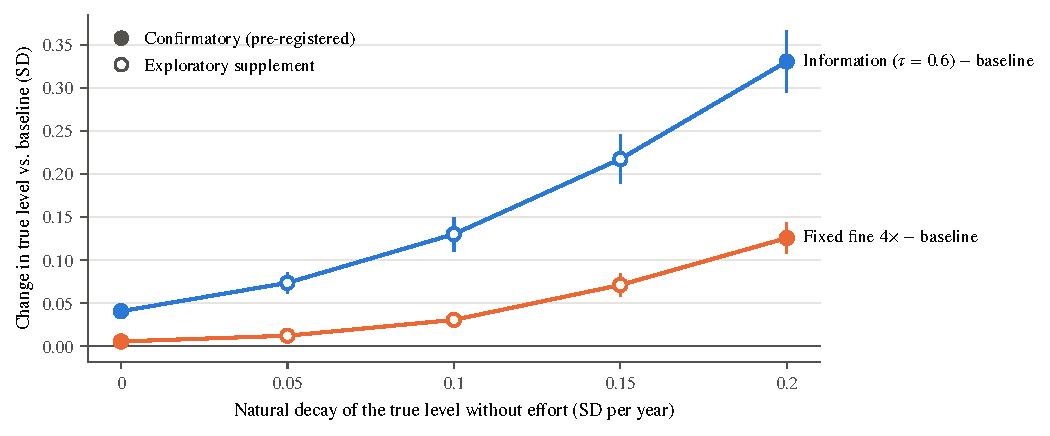
\includegraphics[width=\textwidth]{figures/fig_decay.pdf}
\caption{Policy effects on the true level over the policy window (days 1200--3500) at five uniform rates of natural decay. Points are means over 30 paired seeds; bars are paired 95\% $t$ intervals. Filled points are confirmatory; hollow points come from the exploratory decay supplement.}
\label{fig:decay}
\end{figure}

We therefore report magnitudes as the range from no decay to 0.2~SD per year. Results available only for the main setting --- doses, proportional fines, size and the phase diagrams --- hold under the assumption of 0.2~SD per year and are cited with that condition. The three main contrasts grow with decay, but we have not tested how these other results vary with it, so we do not claim they are upper bounds. Absolute levels are not interpretable: under the assumed decay every scenario declines (B by $-1.196$~SD), and with market preference switched off the decline, $-1.825$~SD, is exactly the decay accumulated over 2,300 days. Only differences between scenarios carry information.

The evidence on decay does not support uniform decay. In a panel of Huazheng ratings of all A-share firms for 2009--2022, which we obtained from a secondary source and have not yet verified against an official export, the average rating has no trend (yearly means between 3.94 and 4.32 on a 1--9 scale), and ratings revert towards the middle: the mean next-quarter change is $+0.30$ notches for the lowest grade and $-0.48$ for the highest. Mean reversion is a different functional form from uniform decay and is not covered by the range above. The panel may not settle the level either: if ratings are relative to peers, an economy-wide trend cannot be seen in them.

\paragraph{Mean reversion (exploratory).} We therefore added a mean-reverting form: the true level reverts towards the day's cross-sectional mean at rate $\kappa$ per year, with idiosyncratic shocks that keep the cross-sectional variance at one, and NPV firms account for the reversion when they value improvement. The panel's quarterly autocorrelation of 0.88 implies $\kappa = 0.50$; removing white-noise measurement error with the ratio of the four-quarter to the one-quarter autocorrelation gives $\kappa = 0.32$. Because the panel's reversion also contains measurement noise and firms' own actions, both are upper bounds on the reversion of the true level. Under both rates the ordering I $>$ F $>$ B survives, but the advantage of information almost disappears. The gap between the instruments is $+0.006$~SD [$+0.004$, $+0.008$] at $\kappa = 0.32$ and $+0.003$ [$+0.002$, $+0.004$] at $\kappa = 0.50$, and the effect of information against the baseline is $+0.027$ and $+0.021$. Both lie below the lower end of the uniform-decay range by amounts the paired intervals resolve. The fixed-fine effect, $+0.021$ and $+0.018$, stays inside it. The mechanism is the one Proposition~\ref{prop:threshold} predicts. Reversion erodes real improvement (half-lives of 1.4--2.2 years) while inflation is removed only by audits, so $A_r$ falls from 3.73 to 2.01 and 1.51 years, and the threshold at $w = 0.2$ rises to 0.77 and 0.82. Transparency of 0.6 no longer stops inflation: 20--22\% of decisions still inflate under I, against 25--28\% under B, so transparency acts much like a heavier fine. Reversion is thus not a decay rate between the two ends of the range. Like no decay, it does not pull the average down; like strong decay, it makes room for inflation; and it lowers the value of real improvement.

\subsection{Investor preference is necessary}\label{sec:preference}

Impact investors' taste raises the true level over the full period by $+0.795$~SD [$+0.743$, $+0.847$] (P1, Holm $p = 3\times10^{-23}$; Table~\ref{tab:primary}). With taste switched off, firms take no action under any policy: improvement earns nothing and inflation is not needed to hold the signal, so the four policies produce identical worlds. The interaction P3, $+0.331$ [$+0.295$, $+0.366$], therefore equals the effect of IF with the market on. It is mechanical rather than a finding about how two forces combine: in this model, policy acts only through the preference of investors.

\begin{table}[t]
\centering
\small
\begin{threeparttable}
\caption{Primary questions}
\label{tab:primary}
\begin{tabular}{@{}llrcc@{}}
\toprule
Question & Contrast & Mean (SD) & 95\% interval & Holm $p$ \\
\midrule
P1 Market preference & B $-$ market-off B, days 0--3500 & $+0.795$ & [$+0.743$, $+0.847$] & $3\times10^{-23}$ \\
P2 Instrument comparison & I $-$ F & $+0.205$ & [$+0.176$, $+0.235$] & $1\times10^{-14}$ \\
P3 Interaction & (IF $-$ B) $-$ (off IF $-$ off B) & $+0.331$ & [$+0.295$, $+0.366$] & $1\times10^{-17}$ \\
P4 Size mechanism & B $-$ equal-cost B, large $-$ small & $+0.229$ & [$+0.205$, $+0.252$] & $6\times10^{-18}$ \\
\bottomrule
\end{tabular}
\begin{tablenotes}[flushleft]\footnotesize
\item \textit{Notes:} Main setting (natural decay 0.2~SD per year), 30 paired seeds. Contrasts P2--P4 use the policy window, days 1200--3500. One run in each of I and IF triggered the price guard; excluding them gives P2 $= +0.207$ and P3 $= +0.333$.
\end{tablenotes}
\end{threeparttable}
\end{table}

Taste with a positive impact-investor share always produced a mixed state under the baseline policy: in every such cell of phase diagram 1 the dominant state was mixed, with decay-adjusted improvement and inflation both above 0.25~SD, and no cell reached improvement without inflation. The investor population itself moves slowly. Over 14 years the impact-investor share rises by only a few percentage points (Section~\ref{sec:model}), so the transition depends on the preference that investors already have rather than on the market recruiting new impact investors.

\subsection{Information versus enforcement}\label{sec:instruments}

Table~\ref{tab:policies} summarises the four main policies. Information beats enforcement by $+0.205$~SD [$+0.176$, $+0.235$] (P2), and both beat the baseline. Across the decay range, the gap is $+0.035$ to $+0.205$~SD. The information policy stops inflation altogether and, because baseline spending goes largely into inflation, firms spend \emph{less} on ESG under it (2.57 against 3.77 basis points of initial market value). Fines collected are tiny, 0.03--0.14 basis points of initial value: fines work through deterrence, not through the money they move.

\begin{table}[t]
\centering
\small
\begin{threeparttable}
\caption{Main policies, policy window}
\label{tab:policies}
\begin{tabular}{@{}lrcrrr@{}}
\toprule
Scenario & True change & Inflating decisions & Mean inflation & Spending & Fines \\
 & (SD) & all (large / mid / small) & (SD) & (bp) & (bp) \\
\midrule
B Baseline & $-1.196$ & 22.3\% (66 / 41 / 6) & 0.95 & 3.77 & 0.05 \\
I Information, $\tau = 0.6$ & $-0.865$ & 0 & 0.43 & 2.57 & 0.03 \\
F Fixed fine $4\times$ & $-1.070$ & 13.3\% (54 / 22 / 2) & 0.77 & 2.98 & 0.14 \\
IF Both & $-0.865$ & 0 & 0.43 & 2.57 & 0.13 \\
Market off (all four) & $-1.825$ & 0 & 0 & 0 & 0 \\
\bottomrule
\end{tabular}
\begin{tablenotes}[flushleft]\footnotesize
\item \textit{Notes:} Means over 30 seeds; main setting. True change is negative in every scenario because of the assumed decay of 0.2~SD per year; only differences between rows are interpretable. Spending is firms' resource cost of improvement and inflation, and fines are fines paid, both in basis points of initial total market value.
\end{tablenotes}
\end{threeparttable}
\end{table}

Figure~\ref{fig:frontier} places every tested dose of each instrument in one plane: the share of decisions that inflate against the change in the true level relative to the baseline. Transparency of 0.3 and 0.5 raises the true level by $+0.181$ and $+0.259$~SD; from 0.6 on, inflation stops and further transparency adds almost nothing ($+0.331$ to $+0.340$). Fixed fines of 2, 4 and 8 times the statutory maximum raise it by $+0.088$, $+0.125$ and $+0.143$, and the share of inflating decisions falls to 15.5\%, 13.3\% and 12.5\%. Within the tested range, no fine dose pushes inflation below 12.5\%, while transparency at or above 0.6 eliminates it. This statement does not depend on how the two doses are matched, but it does depend on per-case booking: once a firm carries an undetected case, new inflation joins it and no fixed fine is added, so higher fines can only stop firms from opening new cases (Proposition~\ref{prop:fixed}).

\paragraph{A fine for every false report (exploratory).} The plateau is an artefact of that accounting. When every false report is fined separately from day~0, and NPV firms charge each new inflation its expected fine, the share of inflating decisions falls from 14.3\% at the statutory fine to 6.6\%, 2.4\% and 0.8\% at 2, 4 and 8 times it. Under per-case booking the corresponding shares are 22.3\%, 15.5\%, 13.3\% and 12.5\%. Deterrence still diminishes: each doubling adds $+0.094$, $+0.064$ and $+0.034$~SD, and each step is smaller than the last by an amount the paired intervals resolve. It diminishes because each doubling deters fewer and larger firms, for which the fine is a smaller share of value; the remaining inflation comes from the largest firms. The fine becomes a stronger instrument ($+0.158$~SD against the baseline, from $+0.125$), the baseline itself improves, and information is unaffected because it stops inflation outright. The gap between information and the quadrupled fine therefore shrinks from $+0.205$ to $+0.058$~SD [$+0.042$, $+0.074$], still positive. Which booking is right is a legal question: several years of false disclosure are often handled in a single penalty decision, but a separate fine per false report is also a plausible reading of the law.

\begin{figure}[t]
\centering
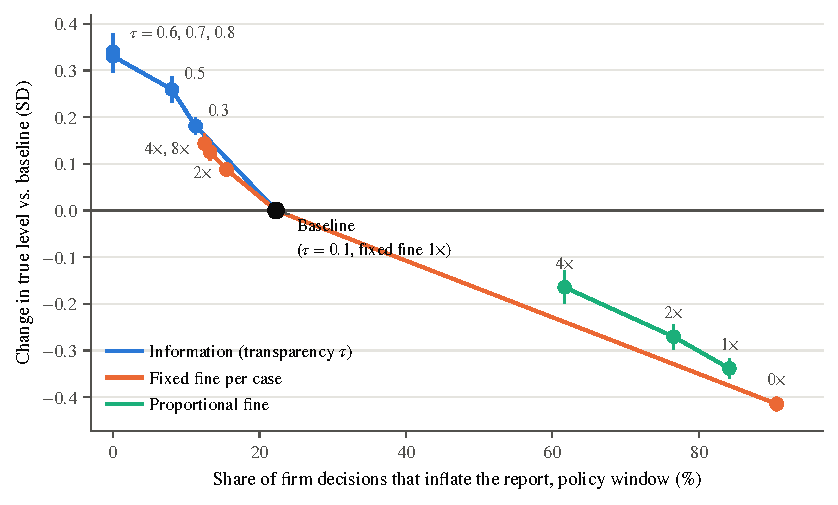
\includegraphics[width=\textwidth]{figures/fig_frontier.pdf}
\caption{Every tested dose of the three instruments: share of firm decisions in the policy window that inflate the report, against the change in the true level relative to the baseline (paired 95\% intervals). The baseline is transparency 0.1 with the statutory fixed fine. Main setting.}
\label{fig:frontier}
\end{figure}

The comparison is a comparison at fixed doses. It is not a comparison at equal expected penalty --- transparency imposes no penalty --- nor at equal social cost, because the costs of standards, assurance and audits are not modelled.

\subsection{The transparency threshold}\label{sec:threshold}

Figure~\ref{fig:threshold} shows the share of inflating decisions on the grid of washing cost ratios and transparency levels, with the threshold $\tau^*(w)$ predicted by Proposition~\ref{prop:threshold}. In all 16 cells the prediction holds: no decision inflates once $\tau \ge \tau^*(w)$, and some do below it. Below the threshold the share declines gradually with transparency, because fines spread firm thresholds. Inflation already in reports does not vanish at the switch: at $w = 0.2$, terminal-year inflation is 1.33~SD at the baseline transparency of 0.1 and 0.35~SD at 0.6, not zero, since only audits, at 1\% per period, or real improvement remove old inflation. Phase diagram 2 has a region of real improvement only where washing is expensive ($w = 0.4$) and transparency is at least 0.6: in each of these two cells, 27 of the 29 classified seeds are real improvement (one seed per cell failed core validation and is not classified).

\begin{figure}[t]
\centering
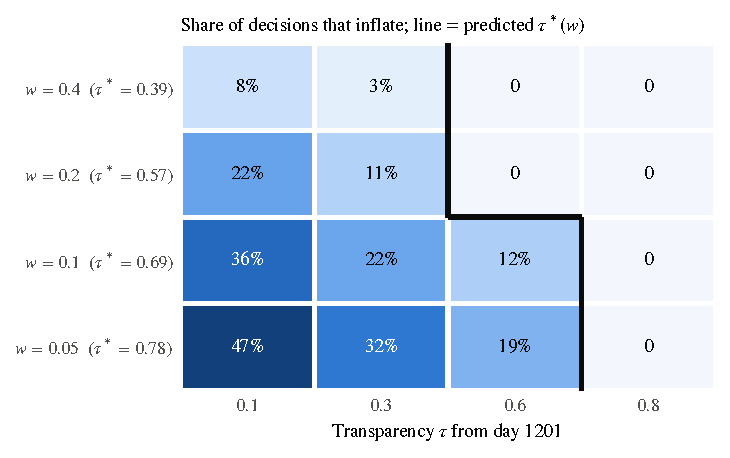
\includegraphics[width=0.78\textwidth]{figures/fig_threshold.pdf}
\caption{Share of firm decisions in the policy window that inflate the report, by washing cost ratio $w$ and transparency $\tau$ (means over 30 seeds). The black line marks the threshold $\tau^*(w)$ of Proposition~\ref{prop:threshold}; the prediction is that no firm inflates to the right of it. Main setting.}
\label{fig:threshold}
\end{figure}

Three qualifications matter for how this result is used. First, as Section~\ref{sec:benchmark} explains, the upper bound of the threshold depends only on $w$ and timing, which the market cannot move; the 16 of 16 match confirms that the simulation implements the rule under feedback, not that real firms behave this way. Second, the threshold is sharp because every firm has the same washing cost ratio. If the ratio differs across firms, the aggregate response is governed by those that inflate most cheaply: in the cells with $w = 0.05$, 19\% of decisions still inflate at $\tau = 0.6$, and inflation stops only near 0.78. Third, the threshold assumes that real improvement lasts. Under mean reversion it rises to about 0.8 (Section~\ref{sec:decay}).

\paragraph{Firm-specific washing costs (exploratory).} We drew each firm's ratio $w_i$ from a lognormal distribution with mean 0.2 and log-SD $\ln 2$ (5th to 95th percentile 0.05 to 0.49). Inflation then no longer stops at a common threshold. At $\tau = 0.6$, 7.3\% of decisions still inflate (none with a common ratio), in every seed. At $\tau = 0.8$, 0.4\% do, in 29 of 30 seeds. The decline is governed firm by firm: all 53,015 inflating decisions after the switch, across the three transparency levels, came from firms whose own threshold $\tau^*(w_i)$ exceeded the current $\tau$, as Proposition~\ref{prop:threshold} implies. The policy comparison barely moves. Information beats the baseline by $+0.320$~SD (common ratio $+0.331$) and the fine by $+0.202$ ($+0.205$). The plateau above $\tau = 0.6$ in Figure~\ref{fig:frontier} partly reflects the common ratio: with dispersed ratios, raising transparency from 0.6 to 0.8 still cuts inflation from 7.3\% to 0.4\%.

\subsection{Fine design and the size divide}\label{sec:size}

The size statistic in this section is the large-minus-small difference in the \emph{change} of the true level over the policy window, days 1200--3500; it says which firms improve more during the window, not how firms rank at its end. Under the baseline, the true level of large firms changes by 0.33~SD less than that of small firms, because large firms inflate in 66\% of their decisions and small firms in 6\%. The fine is the reason: CNY~10 million is a negligible share of a large firm's value, so large firms cross the value threshold $P^*$ of Proposition~\ref{prop:fixed} first. The cost advantage assumed for large firms works the other way. Removing it widens the difference from $-0.33$ to $-0.56$~SD (P4: $+0.229$ [$+0.205$, $+0.252$]), so the difference comes from inflation, not from costs. Under the information policy the sign changes: large firms' true level changes by 0.38~SD \emph{more} than small firms' over the window.

\begin{figure}[t]
\centering
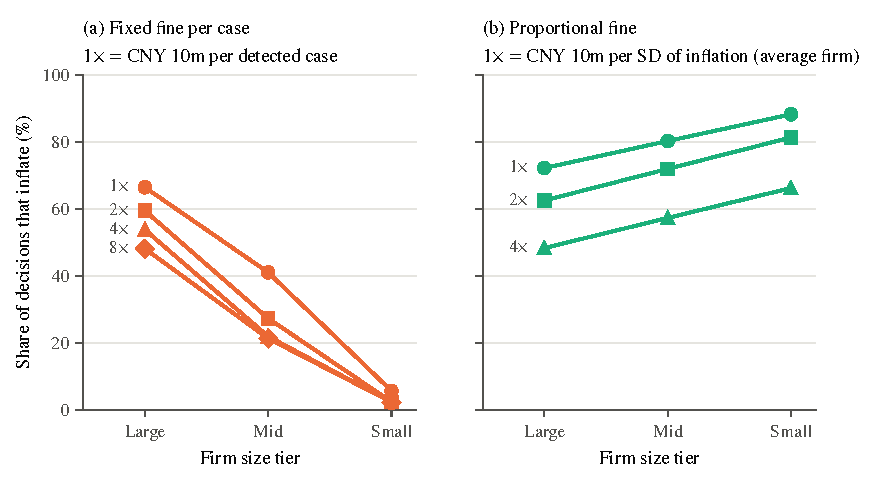
\includegraphics[width=\textwidth]{figures/fig_size.pdf}
\caption{Share of decisions that inflate by firm size tier, under fixed fines per case (a) and under fines proportional to market value and inflation (b), at the doses tested. Labels give the dose as a multiple of the reference. Main setting.}
\label{fig:size}
\end{figure}

Figure~\ref{fig:size} contrasts the two fine designs. Raising the fixed fine eightfold lowers inflation in every tier but still leaves large firms inflating in 48\% of their decisions (66\% at the statutory fine). A proportional fine reverses the size pattern, as Proposition~\ref{prop:fixed} predicts: large firms now inflate least (72\% against 88\% for small firms at $1\times$). But at the equal-amount reference it is much weaker overall. It leaves 84\% of decisions inflating and lowers the true change relative to the fixed fine of the same multiple by $-0.338$~SD [$-0.359$, $-0.318$] at $1\times$, $-0.358$ at $2\times$ and $-0.290$ at $4\times$. The reason is the reference point: per-period inflation is far below 1~SD, so a fine of CNY~10 million per SD of inflation is much lighter per decision than a lump sum of the same amount. The result shows how the two designs differ at this reference; it does not show that either is stronger in general.

\subsection{What the market adds}\label{sec:feedback}

A firm's decision depends on other firms and on investors only through its financing gain $B_i$ and its market value $P_i$, and audit draws come from a separate random stream shared across scenarios. Given the paths of $B$ and $P$ and the audit draws, the firm layer can therefore be replayed without the market. Replaying each run on its own paths reproduces it bit for bit (360 of 360). Replaying a policy scenario on the \emph{baseline} run's paths gives the policy effect without feedback, and the difference from the full model is the contribution of feedback from policy to prices, financing gains and the investor population.

In the main setting this feedback is small and its sign differs by contrast (Table~\ref{tab:feedback}). Its net effect on the information policy cannot be distinguished from zero ($-0.008$~SD [$-0.022$, $+0.007$]). It strengthens the fixed-fine effect by 11\% of that effect ($+0.014$~SD) and narrows the gap between the instruments by 10\% ($-0.021$~SD). The equal-cost and no-decay settings give shares of the same order (10--13\% where identifiable). Where investor taste is doubled, feedback strengthens the fixed-fine effect by 31\% and narrows the gap by 18\%. Freezing the investor population splits the feedback into two channels. In the main setting, investor evolution weakens the information policy ($-0.040$~SD [$-0.054$, $-0.026$], $-12\%$ of its effect), while price and demand responses strengthen it ($+0.032$ [$+0.028$, $+0.037$], $+9.8\%$); the two nearly cancel, and the information policy leaves the impact-investor share 2.0 percentage points lower at the end. The ordering I $>$ F $>$ B holds in 30 of 30 seeds with and without feedback.

\begin{table}[t]
\centering
\small
\begin{threeparttable}
\caption{Contribution of market feedback to policy effects (true change, SD)}
\label{tab:feedback}
\begin{tabular}{@{}lrrrr@{}}
\toprule
 & \multicolumn{2}{c}{Main setting} & \multicolumn{2}{c}{Taste doubled (0.145), II share 0.2} \\
\cmidrule(lr){2-3}\cmidrule(lr){4-5}
Contrast & Feedback & Share of effect & Feedback & Share of effect \\
\midrule
I $-$ B & $-0.008$ & not identified & $-0.024$ & $-4\%$ \\
F $-$ B & $+0.014$ & 11\% & $+0.049$ & 31\% \\
I $-$ F & $-0.021$ & $-10\%$ & $-0.073$ & $-18\%$ \\
\bottomrule
\end{tabular}
\begin{tablenotes}[flushleft]\footnotesize
\item \textit{Notes:} Feedback is the full-model effect minus the effect when the firm layer is replayed on the baseline run's financing gains and market values. Exploratory supplements; 30 paired seeds.
\end{tablenotes}
\end{threeparttable}
\end{table}

The market matters more through the \emph{level} of financing gains it produces than through feedback. Replaying the firm layer on a single snapshot of $B$ and $P$ taken at day 1200, as the browser version of the model does, reproduces the five qualitative patterns we checked but overstates several magnitudes by 27--71\%. The honest summary is that the qualitative results follow from the firms' decision rule, which Section~\ref{sec:benchmark} describes. The artificial market supplies the financing gains that set the magnitudes. Its feedback strengthens fixed fines, narrows the gap between the instruments, and has no identifiable net effect on transparency in the main setting.

\subsection{Learning firms}\label{sec:learning}

We also replaced the NPV rule with tabular Q-learning on realised 60-day accounts: the change in financing fees minus resource costs and fines, scaled by initial value. After fixing what could be fixed --- seven options (three sizes each of improvement and inflation, plus maintaining), polynomial step sizes \citep{evendar2003learning}, a state that carries the firm's own signal tercile, a per-period budget, and contract-scale training worlds --- the learners still failed the pre-set coverage test in the post-policy large-firm group. More importantly, two tables trained independently in the same environment inflated in about 69\% and 15\% of decisions, so the learners' policy ordering cannot be separated from training randomness, and they were excluded from the confirmatory experiment.

A diagnosis with randomly assigned actions points to the size of the signal. At the calibrated premium, the median value of the best action over maintaining is about 0.07 basis points of initial market value (0.52 at the 90th percentile). Within a state, the discounted reward over the following 20 periods, the horizon over which an action's financing effects arrive, has an SD of about 190 basis points. As a rough diagnostic, a two-sample test with that noise would need about $1.2\times10^{8}$ samples per state and action to tell the median value difference apart from zero, and about $2\times10^{6}$ at the 90th percentile, against $10^3$--$10^4$ in our training archives. These figures indicate orders of magnitude; they are not the sample requirement of any particular learning algorithm. Even the one-period reward of maintaining, net of common shocks, has an SD of 2.1 basis points. In addition, the state does not record improvements in progress, so one-step updates credit a delayed financing gain to whatever action happens to be taken when it arrives.

This is a statement about this learner in this calibration, not about real firms. Firms can value ESG through forward-looking appraisal, as our NPV firms do, and through information other than their own accounts. One hypothesis, which our experiments do not test, is that a learner of this kind picks up the quick payoff of inflation more easily than the delayed payoff of improvement, and so drifts towards greenwashing. Testing it would need several independently trained tables per scenario and a control in which the state reveals improvements in progress.

%======================================================================
\section{Robustness and threats to validity}\label{sec:validity}
%======================================================================

Table~\ref{tab:robust} collects the three main contrasts across every setting we ran. The ordering I $>$ F $>$ B holds in all of them, and excluding runs that triggered the price guard changes no verdict. The \emph{size} of the information advantage does not travel. It ranges from $+0.003$ to $+0.224$~SD and depends mainly on two assumptions: that real improvement lasts, and that a fine is charged once per case. A firm-specific washing cost leaves the contrasts in place but removes the sharp threshold. We therefore state the main result as an ordering that is robust across the settings tested, with a magnitude that is not.

\begin{table}[t]
\centering
\small
\begin{threeparttable}
\caption{Policy contrasts across all settings (true change over the policy window, SD)}
\label{tab:robust}
\begin{tabular}{@{}llrrr@{}}
\toprule
Setting & Status & I $-$ B & F $-$ B & I $-$ F \\
\midrule
Uniform decay 0.2 SD/year (main) & Pre-registered & $+0.331$ & $+0.125$ & $+0.205$ \\
No decay & Pre-registered & $+0.040$ & $+0.005$ & $+0.035$ \\
Uniform decay 0.05 SD/year & Exploratory & $+0.073$ & $+0.012$ & $+0.061$ \\
Uniform decay 0.1 SD/year & Exploratory & $+0.130$ & $+0.030$ & $+0.100$ \\
Uniform decay 0.15 SD/year & Exploratory & $+0.217$ & $+0.071$ & $+0.146$ \\
Mean reversion, $\kappa = 0.32$ & Exploratory & $+0.027$ & $+0.021$ & $+0.006$ \\
Mean reversion, $\kappa = 0.50$ & Exploratory & $+0.021$ & $+0.018$ & $+0.003$ \\
A fine for every false report & Exploratory & $+0.216$ & $+0.158$ & $+0.058$ \\
Firm-specific washing cost & Exploratory & $+0.320$ & $+0.118$ & $+0.202$ \\
Equal cost multipliers & Pre-registered & $+0.362$ & $+0.146$ & $+0.216$ \\
Size--ESG independence & Pre-registered & $+0.350$ & $+0.126$ & $+0.224$ \\
Book-equity dispersion & Pre-registered & $+0.269$ & $+0.089$ & $+0.180$ \\
Main setting, new seeds & Second experiment & $+0.318$ & $+0.127$ & $+0.191$ \\
\bottomrule
\end{tabular}
\begin{tablenotes}[flushleft]\footnotesize
\item \textit{Notes:} Means of 30 paired seeds; every paired 95\% interval excludes zero. Rows other than the decay rows use 0.2~SD per year of uniform decay, except the mean-reversion rows, which replace it. Exploratory rows were designed after the confirmatory results and pre-registered before their own runs (contract Sections 20.16 and 20.21). The last row reruns B, I and F on the 30 seeds of the targeted-audit experiment (Section~\ref{sec:targeted}).
\end{tablenotes}
\end{threeparttable}
\end{table}

\paragraph{What remains untested.} The mean-reversion rates are upper bounds from an unverified panel; rates between 0 and 0.32, reversion combined with decay, and firms that ignore reversion were not run. The per-report booking was tested only in the main setting.

\paragraph{Costs and scope of policy.} Neither the cost of transparency nor that of audits is modelled, so the comparison is not about social cost. In the first experiment the regulator does not choose whom to audit and audit intensity is fixed at 1\% per period; Section~\ref{sec:targeted} tests two targeted rules and a doubled budget. There are no assurance providers or rating agencies.

\paragraph{The financing channel.} With the calibrated taste, the local response of a firm's financing rate to its signal --- the quantity firms decide on --- is about 2.2 basis points per SD, an order of magnitude below the empirical cost-of-equity association, because of the reduced-form financing contract. We did not adjust the contract to close the gap, since its parameters are not estimated.

\paragraph{Firm rationality.} Firms are myopic NPV maximisers. Learning firms could not be trained (Section~\ref{sec:learning}), so the results say nothing about boundedly rational firms.

\paragraph{Data.} The CSI~300 contains only large firms and is observed at its current composition. A rating is a proxy, not the true attribute, and the date on a rating need not be the date it became public.

\paragraph{Market layer.} In a qualification audit of 60 fixed worlds, 57 passed and 3 failed mechanical checks; 37 confirmatory runs triggered the price guard; and the simulated-moments fit leaves lag-1 return autocorrelation too negative ($-0.18$ against $-0.03$). All are kept in the record, and the main contrasts do not change when the affected runs are excluded.

%======================================================================
\section{Targeted audits: a second pre-registered experiment}\label{sec:targeted}
%======================================================================

In every run so far the regulator audits each firm with probability 1\% per period. Two results of the first experiment make the allocation of audits worth testing. The statutory fine is negligible for large firms, which inflate in 66\% of their decisions, and a firm with an open case continues to inflate whatever the fine (Section~\ref{sec:benchmark}). Unlike the fine, the audit probability sets both how long inflation survives ($A_w$) and the discounted value of paying on detection ($D$), so it also reaches firms that continue. We therefore ask whether auditing some firms more and others less, at an unchanged expected number of audits, does better than random audits, and whether it matters that firms know the rule.

\paragraph{Design.} The design was written into the research contract (Section~21) and committed (\texttt{962d1ee}) before implementation and runs; the pipeline checks, the frozen configuration (experiment ID \texttt{06bec148\ldots2a32}) and the analysis script were committed (\texttt{3fced38}) before the confirmatory run. The experiment uses 30 new seeds, 42001--42030, and reruns B, I and F on them. On each audit date firm~$i$ is audited if a uniform draw falls below its audit probability $q_i$. The draws are shared across scenarios, and every targeted rule keeps $\sum_i q_i = 2$, the expected number of audits when each of the 200 firms is audited with probability 1\%. The rules are:
\begin{itemize}[leftmargin=*]
\item \emph{Random} (B): $q_i = 1\%$.
\item \emph{By value} (V): $q_i$ is proportional to market value. At the initial distribution of values the median small firm is audited with probability 0.41\% per period, the median large firm 3.0\% and the largest firm 8.0\%.
\item \emph{By jump} (J): half the budget is spread evenly ($q_i = 0.5\%$) and the other half is shared among flagged firms, those whose report (true level plus inflation, before the transparency discount) rose by more than $h = 0.125$~SD, half the per-period cap, since the previous audit date. The random half leaves no firm unaudited.
\item \emph{Doubled random audits} (A2): $q_i = 2\%$, twice the budget, as a reference for auditing more.
\end{itemize}
When a rule is public, firms decide with their own audit probability: under V with the day's $q_i$, under J by predicting whether new inflation will be flagged and choosing the better of staying below the threshold and accepting the flag. When it is hidden (\Vh, \Jh), firms decide as in the first experiment, so targeting changes only who is caught. Firms under J ignore the effect of a flag on older undetected inflation, which understates the cost of being flagged and therefore evasion. The 15 scenarios are B, I, F, A2, V, \Vh, J, \Jh{} and VF (value targeting with the fixed fine at four times the statutory maximum) in the main setting, and B, I, V, J, \Jh{} and VF without natural decay. Five primary questions were tested two-sided with the Holm correction (Table~\ref{tab:audit_primary}), and five analytical predictions derived from the propositions were written down with the design; all five held. All 450 runs completed; five triggered the price guard, all on one seed at day 3101 and none in a scenario of the primary questions.

\begin{table}[t]
\centering
\small
\begin{threeparttable}
\caption{Primary questions of the targeted-audit experiment}
\label{tab:audit_primary}
\begin{tabular}{@{}llrcc@{}}
\toprule
Question & Contrast & Mean (SD) & 95\% interval & Holm $p$ \\
\midrule
E1 Value targeting & V $-$ B & $-0.191$ & [$-0.222$, $-0.159$] & $8\times10^{-13}$ \\
E2 Jump targeting & J $-$ B & $-0.136$ & [$-0.156$, $-0.116$] & $8\times10^{-14}$ \\
E3 Evasion & J $-$ \Jh & $-0.131$ & [$-0.148$, $-0.114$] & $4\times10^{-15}$ \\
E4 Size divide & V $-$ B, large $-$ small & $+0.617$ & [$+0.551$, $+0.683$] & $3\times10^{-17}$ \\
E5 Information vs.\ targeted fine & I $-$ VF & $+0.156$ & [$+0.127$, $+0.186$] & $1\times10^{-11}$ \\
\bottomrule
\end{tabular}
\begin{tablenotes}[flushleft]\footnotesize
\item \textit{Notes:} Main setting (natural decay 0.2~SD per year), policy window, 30 paired seeds (42001--42030). E3 was predicted to be negative and E4 positive; E1, E2 and E5 had no predicted sign. No run in these scenarios triggered the price guard.
\end{tablenotes}
\end{threeparttable}
\end{table}

\paragraph{Results.} At an equal number of audits, both targeted rules do worse than random audits when firms know the rule (E1, E2), although both find more: 50\% of audits under V and 69\% under J find inflation, against 28\% under random audits (Table~\ref{tab:audit_describe}). Hidden, the same rules leave the equal-weighted true level where random audits leave it: \Vh{}~$-$~B is $-0.005$~SD [$-0.012$, $+0.001$] and \Jh{}~$-$~B is $-0.005$ [$-0.011$, $+0.001$]. The loss therefore comes from firms' response to a known rule, not from detection itself; publishing the jump rule costs $0.131$~SD (E3).

Value targeting moves greenwashing from large to small firms. Large firms' share of inflating decisions falls from 64\% to 47\% and small firms' rises from 5\% to 35\%. The size divide reverses: the large-minus-small difference in the change of the true level moves from $-0.30$ to $+0.32$~SD (E4). Weighted by initial market value, the true level rises ($+0.053$~SD [$+0.043$, $+0.063$]), but small firms are 60\% of all firms, and the equal-weighted level falls. Small firms lose more deterrence than large firms gain. The fine is large relative to small firms' value and small relative to large firms', and the detection discount is strongly concave in the audit probability ($D = 0.455$ at 1\% and 0.87 at 8\%). Measured by the expected discounted fixed fine relative to value, with the average firm under random audits at 1, value targeting lowers the median small firm from 2.46 to 1.37 but raises the median large firm only from 0.34 to 0.53. Nor does it end large firms' open cases. By Proposition~\ref{prop:threshold}, with $A_w$ evaluated at the firm's own audit probability, a firm with an open case stops inflating at $\tau = 0.1$ only if that probability is at least 10.5\% per period. All 81,253 continuing inflations under V came from firms below that rate, and the 313 firm-periods that reached it had none.

Firms evade the jump rule. When the rule is public, 44\% of new inflations are flagged at the next audit date, against 54\% when it is hidden (a difference of $-9.6$ percentage points [$-10.9$, $-8.2$]; $-13.8$ points without decay): firms keep inflation below the threshold. Unflagged firms then face an audit probability of only 0.5\%, and small firms, which the fine deterred under random audits, open more new cases; their share of inflating decisions rises by 8.7 points against \Jh.

Auditing more works where auditing differently does not. Doubling random audits raises the true level by $+0.118$~SD [$+0.103$, $+0.133$] and lowers inflation in every size tier, but large firms still inflate in 54\% of their decisions against 2\% for small firms. Both targeted rules fall far short of it (V~$-$~A2 is $-0.309$~SD and J~$-$~A2 is $-0.254$). Information still beats targeted enforcement with a heavier fine: I~$-$~VF is $+0.156$~SD (E5). Adding value targeting to the quadrupled fine helps little in the equal-weighted level (VF~$-$~F is $+0.034$ [$+0.025$, $+0.044$]) and more when weighted by value ($+0.181$ [$+0.160$, $+0.203$]). On the new seeds the main comparison of the first experiment replicates: I~$-$~F is $+0.191$~SD [$+0.165$, $+0.216$], against $+0.205$ in Table~\ref{tab:primary}. Without natural decay all effects are small and keep their signs (V~$-$~B is $-0.003$~SD, J~$-$~B $-0.008$ and I~$-$~VF $+0.026$), so magnitudes are again read as the range between no decay and 0.2~SD per year (Section~\ref{sec:decay}).

\begin{table}[t]
\centering
\small
\begin{threeparttable}
\caption{Targeted-audit experiment: outcomes and audits by scenario}
\label{tab:audit_describe}
\begin{tabular}{@{}lrrcrc@{}}
\toprule
Scenario & True change & \multicolumn{2}{c}{Inflating decisions (\%)} & Hit rate & Audits received (\%) \\
\cmidrule(lr){3-4}
 & (SD) & all & large / mid / small & (\%) & large / mid / small \\
\midrule
B Random & $-1.193$ & 20.3 & 64 / 37 / 5 & 28 & 9 / 32 / 59 \\
I Information, $\tau = 0.6$ & $-0.875$ & 0 & 0 / 0 / 0 & 18 & 9 / 32 / 59 \\
F Fixed fine $4\times$ & $-1.066$ & 11.6 & 53 / 17 / 2 & 19 & 9 / 32 / 59 \\
A2 Doubled random & $-1.075$ & 13.3 & 54 / 23 / 2 & 21 & 10 / 31 / 59 \\
V By value & $-1.384$ & 37.2 & 47 / 38 / 35 & 50 & 35 / 41 / 23 \\
\Vh & $-1.198$ & 22.2 & 69 / 39 / 6 & 54 & 36 / 42 / 23 \\
J By jump & $-1.329$ & 32.5 & 75 / 56 / 14 & 69 & 13 / 42 / 45 \\
\Jh & $-1.198$ & 21.2 & 65 / 39 / 5 & 65 & 16 / 45 / 39 \\
VF Value, fixed fine $4\times$ & $-1.031$ & 10.8 & 28 / 16 / 5 & 32 & 36 / 42 / 23 \\
\bottomrule
\end{tabular}
\begin{tablenotes}[flushleft]\footnotesize
\item \textit{Notes:} Means over 30 seeds; main setting, policy window. The hit rate is the share of audits that find inflation, and audits received is each size tier's share of all audits; the three tiers are 10\%, 30\% and 60\% of firms. B, I and F are rerun on the new seeds, so their values differ slightly from Table~\ref{tab:policies}. True change is negative in every scenario because of the assumed decay; only differences between rows are interpretable.
\end{tablenotes}
\end{threeparttable}
\end{table}

\paragraph{Scope.} The result concerns the two rules tested: a proportional rule, and a jump rule with one threshold, a one-period window and half the budget random. No rule was optimised, so the experiment does not show that targeting cannot beat random audits, only that these two rules do worse once firms know them. The mechanism is reallocation under a fixed budget. Auditing large firms or recent jumps more means auditing small firms or quiet old inflation less, and firms that know the rule inflate where audits thin out. The experiment keeps the other assumptions of the main setting: per-case booking, a common washing cost ratio, uniform decay and fixed doses.

%======================================================================
\section{Conclusion}\label{sec:conclusion}
%======================================================================

In an artificial market calibrated to Chinese magnitudes, raising the transparency of ESG reports did more for firms' true ESG level than raising fixed fines. This held at the doses tested and in every setting we ran: both pre-registered decay rates, three intermediate rates, mean-reverting true levels, a fine for every false report and firm-specific washing costs. It held again on the new seeds of the second experiment, where transparency also beat value-targeted audits combined with the quadrupled fine. How much more depends on two things the model cannot settle. If real improvements fade towards the mean, as the only rating panel we hold suggests, transparency of 0.6 no longer stops greenwashing and its advantage over a quadrupled fine nearly vanishes. If every false report is fined separately, fines lose their deterrence plateau and the gap narrows to a quarter of its main-setting size. Whether fines are booked per case or per report is a question of law and enforcement practice. Whether ESG performance reverts is a question for verified rating data. Both deserve answers before either instrument is preferred on these grounds.

Some results hold across these settings. None of the instruments works without investors who value ESG, and the market's own drive to recruit them is weak. A fine of the size the Securities Law allows is negligible for large firms, where greenwashing concentrates. A fine proportional to value reverses that tilt even at the lowest dose tested, but at the equal-amount reference it leaves 62--84\% of decisions inflating. And with heterogeneous firms, transparency works firm by firm rather than through a single threshold.

The second experiment adds a caution about targeting audits. At an unchanged number of audits, auditing large firms more or auditing firms whose reports jump did worse than random audits once firms knew the rule, because greenwashing moved to where audits thinned out; with the rule hidden, targeting made no difference, and doubling random audits helped. A rule that catches more inflation per audit can still deter less, so a targeting rule has to be judged by how firms respond to it.

The model is a laboratory, not a forecast. Its value lies in making each step from assumption to result inspectable: the analytical benchmark shows which results follow from the firm's decision rule, the feedback decomposition shows how much the market adds, and the pre-registration and archive show what was decided before the results were seen. Verified rating panels, audit rules designed against firms' responses, assurance providers, and firms that learn with enough data are the natural next steps.

\bibliographystyle{plainnat}
\bibliography{references}

\appendix

%======================================================================
\section{Reproducibility}\label{app:repro}
%======================================================================

All code, configurations and evidence are in the public repository \url{https://github.com/kanzaler123/financial-ABM} (MIT licence). Vendor data without a redistribution licence (Huazheng ratings, market data) are not included; collection scripts and hash manifests are.

\begin{itemize}[leftmargin=*]
\item \emph{Pre-registration:} research contract, Section~20 (\path{docs/disclosure_research_contract.md}), committed before the confirmatory run (\texttt{2b08f65}); supplements in Sections 20.16--20.21.
\item \emph{Confirmatory experiment:} configuration \path{configs/disclosure_stage_f_confirmatory_v1.json}, experiment ID \texttt{90ee8606\ldots5d57}, seeds 41001--41030; report \path{reports/disclosure_stage_f_20261014/}.
\item \emph{Supplements} (under \path{reports/}): \path{disclosure_robustness_20261018/} (contract Section 20.21), \path{disclosure_decay_grid_20261016/}, \path{disclosure_feedback_counterfactual_20261016/}, \path{disclosure_feedback_strong_20261016/}, \path{disclosure_feedback_channels_20261017/}, \path{disclosure_feedback_channels_main_20261017/}.
\item \emph{Targeted audits:} research contract, Section~21, committed before implementation and runs (\texttt{962d1ee}); pipeline checks, frozen configuration and analysis script committed before the confirmatory run (\texttt{3fced38}); configuration \path{configs/disclosure_targeted_audits_confirmatory_v1.json}, experiment ID \texttt{06bec148\ldots2a32}, seeds 42001--42030; report \path{reports/disclosure_targeted_audits_20261020/}.
\item \emph{Figures:} \path{python paper/make_figures.py} reads only committed analysis files.
\item \emph{Browser version:} the firm decision rule in the online sandbox matches the Python rule on 1,200 random inputs with a maximum relative error of $1.0\times10^{-14}$.
\end{itemize}

%======================================================================
\section{Additional results}\label{app:extra}
%======================================================================

\begin{table}[h]
\centering
\small
\begin{threeparttable}
\caption{Policy contrasts across settings (true change, SD)}
\label{tab:robustness}
\begin{tabular}{@{}lrrrrr@{}}
\toprule
Contrast & Main & No decay & Equal cost & Size--ESG independent & Book-equity dispersion \\
\midrule
I $-$ B & $+0.331$ & $+0.040$ & $+0.362$ & $+0.350$ & $+0.269$ \\
F $-$ B & $+0.125$ & $+0.005$ & $+0.146$ & $+0.126$ & $+0.089$ \\
I $-$ F & $+0.205$ & $+0.035$ & $+0.216$ & $+0.224$ & $+0.180$ \\
\bottomrule
\end{tabular}
\begin{tablenotes}[flushleft]\footnotesize
\item \textit{Notes:} Policy window, 30 paired seeds; no interval includes zero. The last two columns are the initialisation controls declared before any policy result.
\end{tablenotes}
\end{threeparttable}
\end{table}

\begin{table}[h]
\centering
\small
\begin{threeparttable}
\caption{Dose responses (true change relative to B, SD; share of decisions that inflate)}
\label{tab:doses}
\begin{tabular}{@{}lrrrrr@{}}
\toprule
Transparency $\tau$ & 0.3 & 0.5 & 0.6 & 0.7 & 0.8 \\
\midrule
Change & $+0.181$ & $+0.259$ & $+0.331$ & $+0.337$ & $+0.340$ \\
Inflating & 11.3\% & 8.0\% & 0 & 0 & 0 \\
\midrule
Fixed fine (multiple) & $0\times$ & $1\times$ (B) & $2\times$ & $4\times$ (F) & $8\times$ \\
\midrule
Change & $-0.414$ & 0 & $+0.088$ & $+0.125$ & $+0.143$ \\
Inflating & 90.6\% & 22.3\% & 15.5\% & 13.3\% & 12.5\% \\
\midrule
Proportional fine (multiple) & $1\times$ & $2\times$ & $4\times$ & & \\
\midrule
Change vs.\ same fixed multiple & $-0.338$ & $-0.358$ & $-0.290$ & & \\
Inflating (large / mid / small) & 72 / 80 / 88\% & 62 / 72 / 81\% & 48 / 57 / 66\% & & \\
\bottomrule
\end{tabular}
\end{threeparttable}
\end{table}

\end{document}
